
\documentclass[a4paper,12pt]{article} % тип документа


% Русский язык
\usepackage[T2A]{fontenc} % кодировка
\usepackage[utf8]{inputenc} % кодировка исходного текста
\usepackage[english,russian]{babel} % локализация и переносы


% Математика
\usepackage{amsmath,amsfonts,amssymb,amsthm,mathtools}


\usepackage{wasysym}

%Заговолок
\author{Талашкевич Даниил Александрович}

\title{Неделя 6. Двудольные графы, паросочетания
и функции}

\date{\today}

\begin{document}

\maketitle
\thispagestyle{empty}

\newpage
\setcounter{page}{1}
\begin{center}
\itshape
\bfseries
{ \Large Problems:}
\end{center}

{\bf 1.} Частичная функция $h$ из множества $\{0, 1, \dots , 8\}$ в множество $\{a, b, \dots, g\}$
определена следующим образом:
\[ h : 1\rightarrow b,2 \rightarrow c, 3 \rightarrow b, 4\rightarrow e, 5 \rightarrow b, 6\rightarrow e, 8 \rightarrow f. \]

Найдите: {\bf a)}Dom($h$); {\bf б)} Range($h$); $h(\{ 0,1,2,3,4\})$; {\bf в)} $h^{-1}(\{ a,b,c\})$.
\begin{center}
\bfseries
{\Large Решение: }
\end{center}

\[1) \text{ } Dom(h) = \lbrace 1, 2, 3, 4, 5, 6, 8 \rbrace\]
\[2) \text{ } Range(h) = \lbrace b, c, e, f\rbrace, \text{ } h(\lbrace 0,1,2,3,4\rbrace) = \lbrace b, c, e \rbrace \]
\[3) \text{ } h^{-1}(\lbrace a,b,c\rbrace) = \lbrace 1,2,3,5 \rbrace\]
\[4) \text{ } h^{-1}(h(\lbrace 0,1,2,6,7,8\rbrace)) = h^{-1}(\lbrace b,c,e,f \rbrace) = \lbrace 1,2,3,4,5,6,8 \rbrace\]
\[5) \text{ } h(h^{-1}(\lbrace a,b,c,d,e\rbrace)) = h(\lbrace 1,2,3,4, 5,6\rbrace) = \lbrace b, c, e \rbrace\]


\begin{flushright}
\begin{large}
\textbf {Ответ: }
\end{large}
\end{flushright}

{\bf 2.} Частичная функция $f$ из множества целых чисел в множество целых
чисел сопоставляет числу $x$ наименьшее простое число, которое больше $x^2$
. Докажите, что если множество целых чисел $X$ конечное, то и
полный прообраз этого множества $f^{-1}(X)$ конечен.
\begin{center}
\bfseries
{\Large Решение: }
\end{center}



Так как прообраз множества равен объединению прообразов его элементов, то необходимым и достаточным будет доказать, что прообраз элемента конечен. Для данного простого $p$ в его прообраз попадают только те элементы $x$, для которых $f(x)=x^2 < p$, то есть $|x| < \sqrt{p}$. Количество таких значений конечно, а значит и полный прообраз множества $f^{-1}(X)$ конечен.


\begin{flushright}
\begin{large}
\textbf {доказано }
\end{large}
\end{flushright}


{\bf 3.} Пусть $f$ -- частичная функция из множества $X$ в множество $Y$ , при
этом $A \subseteq X$.Какой знак сравнения можно поставить вместо «?», чтобы
утверждение \[ f^{-1}(f(A))?A\]

стало верным? (Возможные знаки сравнения в этой и двух следующих
задачах: $\subseteq,\ \supseteq,\ =$ . Нужно учесть все варианты.)
\begin{center}
\bfseries
{\Large Решение: }
\end{center}

Для рассуждения хорошо подходят функция из задачи 1:

\[h(h^{-1}(\lbrace a,b,c,d,e\rbrace)) = h(\lbrace 1,2,3,4, 5,6\rbrace) = \lbrace b, c, e \rbrace\]

Отсюда видно, что не может реализоваться ситуация $f^{-1}(f(A)) \subseteq A$, а отсюда и $f^{-1}(f(A)) = A$. Значит знак в исходном равенстве -- $\supseteq$.

Заметим, что решение справедливо только в том случае, когда функция сюрьективна. Если это не так, то, например:
\[h^{-1}(h(\lbrace 0,1,2,6,7,8\rbrace)) = h^{-1}(\lbrace b,c,e,f \rbrace) = \lbrace 1,2,3,4,5,6,8 \rbrace\]

Видно, что в этом случае равенство не выполняется ни при одном знаке сравнения: $f^{-1}(f(A)) \nsubseteq A$, $f^{-1}(f(A)) \nsupseteq A$, $f^{-1}(f(A)) \neq A$.\\


\begin{flushright}
\begin{large}
\textbf {Ответ: $\supseteq$ для сюрьективных функций, нет решений для не сюрьектвных функций }
\end{large}
\end{flushright}
{\bf 4.} Пусть $f$ -- частичная функция из множества $A \cup B$ в множество. $Y$  Какой знак сравнения можно поставить вместо «?», чтобы утверждение \[ f(A \setminus B) ? f(A) \setminus f(B)\]

стало верным?
\begin{center}
\bfseries
{\Large Решение: }
\end{center}

Из подсказки приведем такой пример, чтобы включение не выполнялось: $A = \{a_1,a_2,a_3\}$, а $B = \{a_3,a_4,a_5\}$. Тогда 

$f : a_1 \rightarrow a, a_2 \rightarrow b, a_3 \rightarrow a, a_4 \rightarrow b, a_5 \rightarrow a.$

$f(A \setminus B) = f(a_1,a_2) = a, b.$

$f(A) \setminus f(B) = \varnothing.$

Отсюда следует, что $f(A \setminus B)$ надмножество множества $f(A) \setminus f(B) \Rightarrow "\supseteq".$

\begin{flushright}
\begin{large}
\textbf {$"\supseteq"$. }
\end{large}
\end{flushright}
{\bf 5.} Пусть $f$ -- частичная функция из множества $X$ в множество $Y$ , при
этом $A \cup B \subseteq Y$ . Какой знак сравнения можно поставить вместо «?»,
чтобы утверждение \[ f^{-1}(A \setminus B ? f^{-1}(A)\setminus f^{-1}B \]

стало верным?
\begin{center}
\bfseries
{\Large Решение: }
\end{center}

\[x \in A \setminus B \Rightarrow x \in A \wedge x \notin B\]
\[f^{-1}(A \setminus B) = \lbrace x \text{ }|\text{ } \exists y \in A : (f(x) = y \in A) \wedge (f(x) \notin B )\rbrace\]
\[f^{-1}(A) = \lbrace x \text{ }|\text{ } \exists y \in A: f(x) = y \in A \rbrace\]
\[f^{-1}(B) = \lbrace x \text{ }|\text{ } \exists y \in B: f(x) = y \in B \rbrace\]
\[f^{-1}(A) \setminus f^{-1}(B) = \lbrace x \text{ }|\text{ } (\exists y \in A: f(x) = y \in A) \wedge (\nexists z \in B: f(x) = z \in B) \rbrace\]

Остаётся сравнить два выражения:
\[f^{-1}(A) \setminus f^{-1}(B) = \lbrace x \text{ }|\text{ } (\exists y \in A: f(x) = y \in A) \wedge (\nexists z \in B: f(x) = z \in B) \rbrace\]
\[f^{-1}(A \setminus B) = \lbrace x \text{ }|\text{ } \exists y \in A : (f(x) = y \in A) \wedge (f(x) \notin B )\rbrace\]

Остаётся заметить, что оба определения через кваннторы эквивалентны, так как в обоих случаях $f(x) \notin B$.  

\begin{flushright}
\begin{large}
\textbf {Ответ: $=$}
\end{large}
\end{flushright}
{\bf 6.} Верно ли, что если каждая вершина графа имеет степень 1 или
2 и в графе нет (простых) циклов нечётной длины, то в графе есть
совершенное паросочетание?
\begin{center}
\bfseries
{\Large Решение: }
\end{center}

Из определения паросочетания (множество рёбер, не имеющих общих концов) получим контрпример дерево из 3 вершин, степени 2, 1, 1.
Циклов нечетной длины нет, а каждая степень графа имеет степень 1 или 2, но паросочетание $\varnothing$.



\begin{flushright}
\begin{large}
\textbf {нет, не верно. }
\end{large}
\end{flushright}
\newpage
{\bf 7.} Про частичная функция $f$ из множества $X$ в множество $Y$ и множество $B \subseteq Y$ известно, что $f^{-1}(B) = X$. Верно ли, что $B = Y$ ?
\begin{center}
\bfseries
{\Large Решение: }
\end{center}

Предположим, что равенство не выполняется и $B \subset Y$. Тогда для любой функции каждому элементу из области определения соответствует только один элемент из области значений функции.

Пусть $\exists y_0: y_0 \in Y \wedge y_0 \notin B $, тогда $\exists x_0: x_0 \in X: f(x_0) = y_0$. Данному $x_0$ соответсвует единственное значение $y_0$, тогда $x_0 \notin f^{-1}(B)$. Полученное проти-
воречие указывает на то, что наше предположение неверно, значит $B = Y$.

(Если функция не является сюръекцией, то утверждение неверно -- пример
приведён в следующем номере.)\\


\begin{flushright}
\begin{large}
\textbf {Ответ: верно для сюрьективных функций, неверно для не сюрьективных функций}
\end{large}
\end{flushright}
{\bf 8.} Приведите пример такой инъекции $f$ из множества $X$ в множество
$Y$ , что для некоторого $B \subseteq Y$ выполняются оба условия

1)$B \neq \varnothing$,

2)$f^{-1} = \varnothing$.
\begin{center}
\bfseries
{\Large Решение: }
\end{center}

Пример очень простой, достаточно взять любую вершину, чтобы множество $B \neq \varnothing$ и $f^{-1}(B) = \varnothing$, тогда будут выполняться оба условия.

\begin{center}
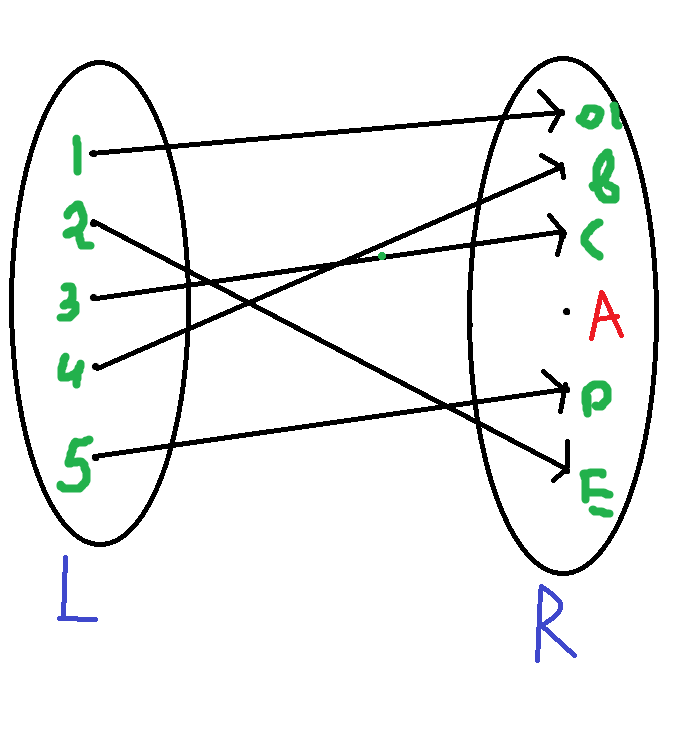
\includegraphics[scale=0.5]{6 1}
пример.
\end{center}

Здесь $ B = {A} \neq \varnothing$ и $f^{-1}(B) = \varnothing$.

\begin{flushright}
\begin{large}
\textbf {приведён пример.}
\end{large}
\end{flushright}
\newpage
{\bf 9.} Постройте биекцию между конечными подмножествами множества

положительных целых чисел и конечными строго возрастающими по-
следовательностями положительных целых чисел.
\begin{center}
\bfseries
{\Large Решение: }
\end{center}

Рассмотрим конечные подмножества множества положительных целых чисел. Обозначим множество таких подмножеств за $X$. В этих подмножествах можно расставить числа таким образом, чтобы в каждом подмножестве числа стояли по возрастанию. Таким образом мы получили конечные строго возрастающие последовательности положительных целых чисел, которые обозначим за $Y$.

Очевидно, что можно построить биекцию из конечных строго возрастающих последовательностей положительных целых чисел в конечные строго возрастающие последовательности положительных целых чисел. Теперь, когда биекция построена, Переставим обратно все числа в подмножествах множества $X$ в таком порядке, в каком они были изначально, при этом биекция сохраняется.

Итак, построили биекцию между конечными подмножествами множества положительных целых чисел и конечными строго возрастающими последовательностями положительных целых чисел.


\begin{flushright}
\begin{large}
\textbf {Доказано }
\end{large}
\end{flushright}
\newpage
{\bf 10.} (Теорема Кёнига) Докажите, что размер максимального паросоче-
тания (число рёбер) в двудольном графе $G$ совпадает с размером его

минимального вершинного покрытия.
\begin{center}
\bfseries
{\Large Решение: }
\end{center}

Пусть задан двудольный граф ${\displaystyle G=(X,Y,E)}$, а $M$ — наибольшее паросочетание в $G$.

Сначала рассмотрим случай, когда паросочетание $M$ насыщает все вершины доли $X$, то есть размер паросочетания $M$ равен $|X|$. Очевидно, что вся доля $X$ является вершинным покрытием в графе $G$, следовательно, она является и наименьшим вершинным покрытием, и в этом случае утверждение теоремы выполняется.

Иначе возьмём все вершины доли $X$, не насыщенные паросочетанием $M$, и запустим из них обход в ширину($\ast$) по следующему правилу:


($\ast$)Поиск в ширину -- один из методов обхода графа. Пусть задан граф $G=(V,E)$ и выделена исходная вершина $s$. Алгоритм поиска в ширину систематически обходит все ребра $G$ для «открытия» всех вершин, достижимых из $s$, вычисляя при этом расстояние (минимальное количество рёбер) от $s$ до каждой достижимой из $s$ вершины. Алгоритм работает как для ориентированных, так и для неориентированных графов.($\ast$)


1. Слева направо переходим только по рёбрам, не входящим в $M$ (будем называть их чёрными).

2. Справа налево переходим только по рёбрам, входящим в $M$ (будем называть их голубыми).

Пусть $X^{+}$ и $Y^{+}$ — подмножества вершин левой и правой доли, посещённых во время обхода, а $X^{-}$ и $ Y^{-}$ — соответственно, подмножества не посещённых вершин (см. рисунок 1).

\begin{center}
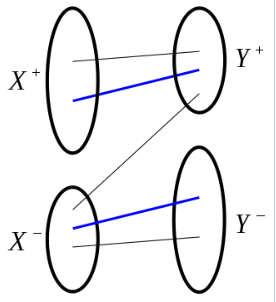
\includegraphics[scale=1]{6 2}

рис. 1
\end{center}

Между множествами $X^{+}$ и $ Y^{-}$ нет чёрных рёбер, поскольку иначе во время обхода мы бы посетили вершины из множества $Y^{-}$. По аналогичной причине, между множествами $X^{-}$ и $Y^{+}$ нет голубых рёбер.

Докажем, что между множествами $ X^{+}$ и $Y^{-}$ нет также и голубых рёбер. От противного, пусть такое ребро $\{x^{+},y^{-}\}$ есть. Вершина $x^{+}$ не могла являться стартовой для обхода в ширину, поскольку она насыщена паросочетанием $M$. Следовательно, обход в ширину пришёл в $x^{+}$ из какой-то вершины $y^{+}$ по голубому ребру, что означает, что вершине $x^{+}$ инцидентны два голубых ребра $\{x^{+},y^{-}\}$ и $\{x^{+},y^{+}\}$. Но это невозможно, поскольку голубые рёбра образуют паросочетание.

Следовательно, любое ребро графа $G$ инцидентно или вершине из $X^{-}$ или вершине из $Y^{+}$, то есть $X^{-}\cup Y^{+}$ является вершинным покрытием. Покажем, что все вершины в $X^{-}\cup Y^{+}$ насыщены паросочетанием $M$. Для вершин из $X^{-}$ -- это очевидно, поскольку все ненасыщенные вершины левой доли по построению лежат в $X^{+}$. Если в$Y^{+}$ есть ненасыщенная вершина, то существует $M$ --чередующая цепь, заканчивающаяся в ней, что противоречит тому, что паросочетание $M$ является наибольшим. Теперь осталось вспомнить, что между множествами $X^{-}$ и $Y^{+}$ нет рёбер из $M$, то есть каждому ребру паросочетания инцидентна в точности одна вершина из вершинного покрытия $ X^{-}\cup Y^{+}$. Следовательно, $|M|=|X^{-}\cup Y^{+}|$, и вершинное покрытие $X^{-}\cup Y^{+}$ является наименьшим.


\begin{flushright}
\begin{large}
\textbf {доказано}
\end{large}
\end{flushright}


{\bf 11.} В прямоугольнике $m\times n$ стоят фишки $m$ разных цветов, по $n$ штук
каждого цвета. Докажите, что можно переставить фишки в каждой
строке так, чтобы в каждом столбце были фишки всех цветов.
\begin{center}
\bfseries
{\Large Решение: }
\end{center}


Будем доказывать по индукции. База: в прямоугольнике $m\cdot 1$ можно переставить фишки в каждой строке так, чтобы в каждом столбце были фишки всех цветов, так как других вариантов расстановки в данном случае нет.

Пусть верно, что прямоугольнике $m\cdot k$ можно переставить фишки в каждой строке так, чтобы в каждом столбце были фишки всех цветов. Докажем, что и прямоугольнике $m\cdot (k + 1)$ можно переставить фишки в каждой строке так, чтобы в каждом столбце были фишки всех цветов.

Рассмотрим самую нижнюю строку прямоугольника, предположим, что она состоит только из фишек одного цвета, тогда этот цвет уже присутствует во всех столбцах, значит переходим к строке выше.

Если же строка состоит не из одного цвета, то как минимум есть 2 цвета. Рассмотрим фишки какого-то из цветов в этой строке. Количество этих фишек не больше $k$, так как строка состоит не из одного цвета. Значит как минимум есть фишки такого же цвета в каких-то других строках. Значит поставим фишку рассматриваемого цвета в рассматриваемой строке в самую правую позицию и больше не будем использовать фишки этого цвета в правом столбце прямоугольника. При этом в других строках, где есть этот цвет, есть также другие цвета, которые мы можем поставить в правую позицию строки.

Проделываем те же операции со строками за исключением того, что теперь в случае не одного цвета в строке мы больше не можем выбрать произвольный цвет, как это сделали для самой первой строки.

Может оказаться, что в расссматриваемой строке есть только цвета, которые уже были использованы до этого в правой позиции строк (последний столбец). В этом случае в правую позицию ставим произвольный цвет из этой строки, возвращаемся к строке, где уже был использован этот цвет в правой позиции, и меняем цвет в правой позиции на этой строке. Если на этой строке возникает такая же проблема, то спускаемся ещё на одну строку, которая была рассматроена перед текущей. Если мы так доходим до самой первой рассматриваемой строки, то выберем другой произвольный цвет у строки на самой верхушке рассматриваемых строк и проделываем те же действия.
Если для всех цветов строки на верхушке рассматриваемых строк остаётся описанная проблема, то на этот раз меняем произвольно выбранный цвет у самой первой строки и проделываем все описанные выше операции. Если же проблема никак не рашается, что есть фишки с каким-то цветом в количестве более, чем $k+1$, что невозможно.

Таким образом мы построили последний столбец, состоящий из $m$ разных цветов. Для рассматриваемого прямоугольника можно построить $k$ столбцов, состоящих из разных цветов, по индукции, а $k+1$ столбец мы только что построили. Значит утверждение для $k+1$ справедливливо и мы доказали требуемое утверждение по индукции.



\begin{flushright}
\begin{large}
\textbf {Доказано}
\end{large}
\end{flushright}


\end{document}


